\documentclass[a4paper,12pt]{article}
\usepackage{lastpage}
\usepackage{epsfig}
\usepackage{graphics}
\usepackage{enumitem}
\usepackage{amsmath}
\usepackage{soul}
\topmargin=-0.5in
\textheight=9.5in
\oddsidemargin=-0.125in
\textwidth=6.75in
\begin{document}

\parindent=24pt
\everymath{\displaystyle}

\def\Letter#1{\ifcase #1\or A\or B\or C\or D\or E\or F\or G\or H\or I\or J\or K\or L\or M\or N\fi}
\def\letter#1{\ifcase #1\or a\or b\or c\or d\or e\or f\or g\or h\or i\or j\or k\or l\or m\or n\fi}

\newcount\n
\def\problem#1#2{% #1: name of the problem; #2: time limit, in seconds
\vfill \newpage
\advance\n by 1
\begin{center}
{\LARGE\bf Problem \Letter\n\quad}\\
\medskip
{\Large\bf #1}\\
\medskip
{\large\bf Time limit: #2 seconds}
\end{center}
\bigskip
}

%=======================================
% Do not modify the above lines.
%=======================================

\problem{Temperature Difference}{10}

Gaia travels among planets via (bidirectional) wormholes. She starts from planet $X$ and plans to reach planet $Y$. There may or may not exist a wormhole that connects planets $X$ and $Y$ directly. Therefore, on some occasions, it is necessary to traverse along a sequence of wormholes rather than just a single one. Some intermediate planets other than $X$ and $Y$ are visited while transferring from one wormhole to another. Given the temperature of all planets, Gaia would like to search for a sequence of wormholes from planet $X$ to $Y$ that minimizes the temperature difference between the hottest visited planets and the coldest visited one. For the sake of simplicity, we assume that planet $X$ has temperature $X$ (K) for each $X$. 

\begin{figure}[!h]
\centering
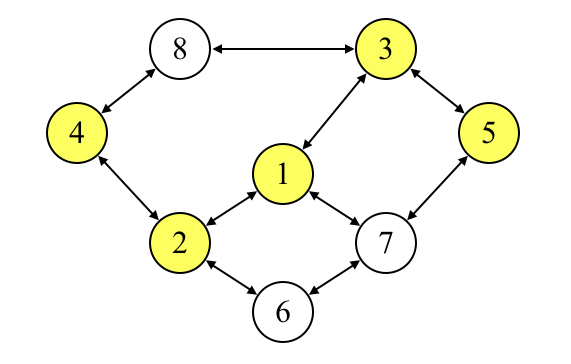
\includegraphics[width=0.6\textwidth]{fig1.png}
\caption{If $X = 4$ and $Y = 5$, then the best route for Gaia to reach $Y$ from $X$ is $4 \rightarrow 2 \rightarrow 1 \rightarrow 3 \rightarrow 5$ because it has the smallest temperature difference $4$. \label{fig:drawing}}
\end{figure}


%\section*{Technical Specification}
%\begin{enumerate}
%\item There are at most 40 testcases.
%\end{enumerate}


\section*{Input Format}

In the first line, three integers $n, m, k$ are given. $n$ is an integer in $[1, 3000]$ that denotes the number of planets, and $m$ is an integer in $[1, n(n-1)/2]$ that denotes the number of wormholes. $k$ is an integer in $[1, 20]$ that specifies the number of queries. The $n$ planets are numbered from $1$ to $n$. Then the description of the $m$ wormholes follows. Each wormhole is specified by the identifier of the end-planets, $u$ and $v$ for some $u \ne v \in \{1, 2, \ldots, n\}$. Then the description of the $k$ queries follows. Each query gives an $(X, Y)$ pair. You may assume that the planets are connected.

\section*{Output Format}

For each query, output the smallest temperature difference on a unique line.

\section*{Sample Input}
\begin{verbatim}
8 10 3
4 8 8 3 3 5
4 2 2 1 1 7 7 5
2 6 6 7
1 3
4 5
1 6
8 8
\end{verbatim}

\section*{Sample Output for the Sample Input}
\begin{verbatim}
4
5
0
\end{verbatim}


\vfill \newpage

\begingroup
\catcode`@ = 11
\protected@write\@auxout{}{\string\newcount\n \n=\the\n}
\endgroup

\end{document}
